\documentclass[11pt]{article}
\usepackage{textcomp}
\usepackage{fontenc}

\usepackage{graphicx}
\usepackage{caption}
\usepackage{sidecap}
\usepackage{enumitem}
\usepackage{multicol}
\usepackage{gensymb}
\usepackage{placeins}
\setlength{\parskip}{3 mm}

\graphicspath{{images/}}	% Root directory of the figures

\title{Community Dyanmics meta analysis - Draft}

\renewcommand*{\familydefault}{\sfdefault}



\begin{document}

\maketitle
% \section{Abstract}


% \section{Introduction}

% \section{Materials and Methods}


\section{Results}


Overall relationship between spatial and temporal heterogeneity

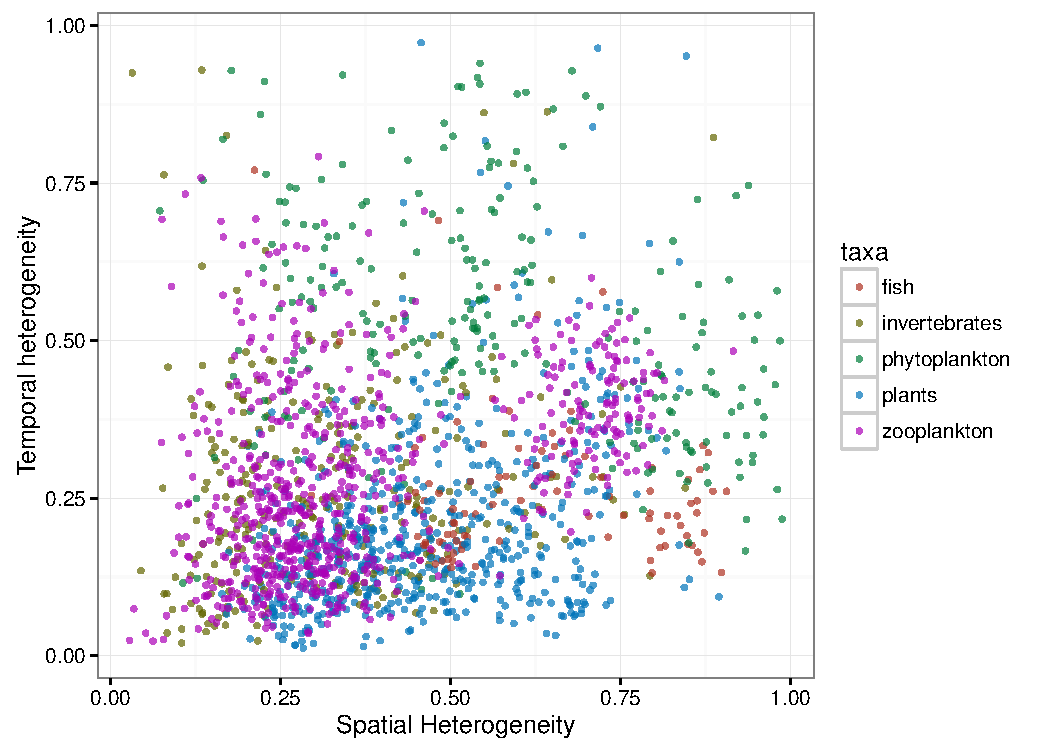
\includegraphics[width=400px]{overall}


\newpage
Overall relationship, aggregated by study.

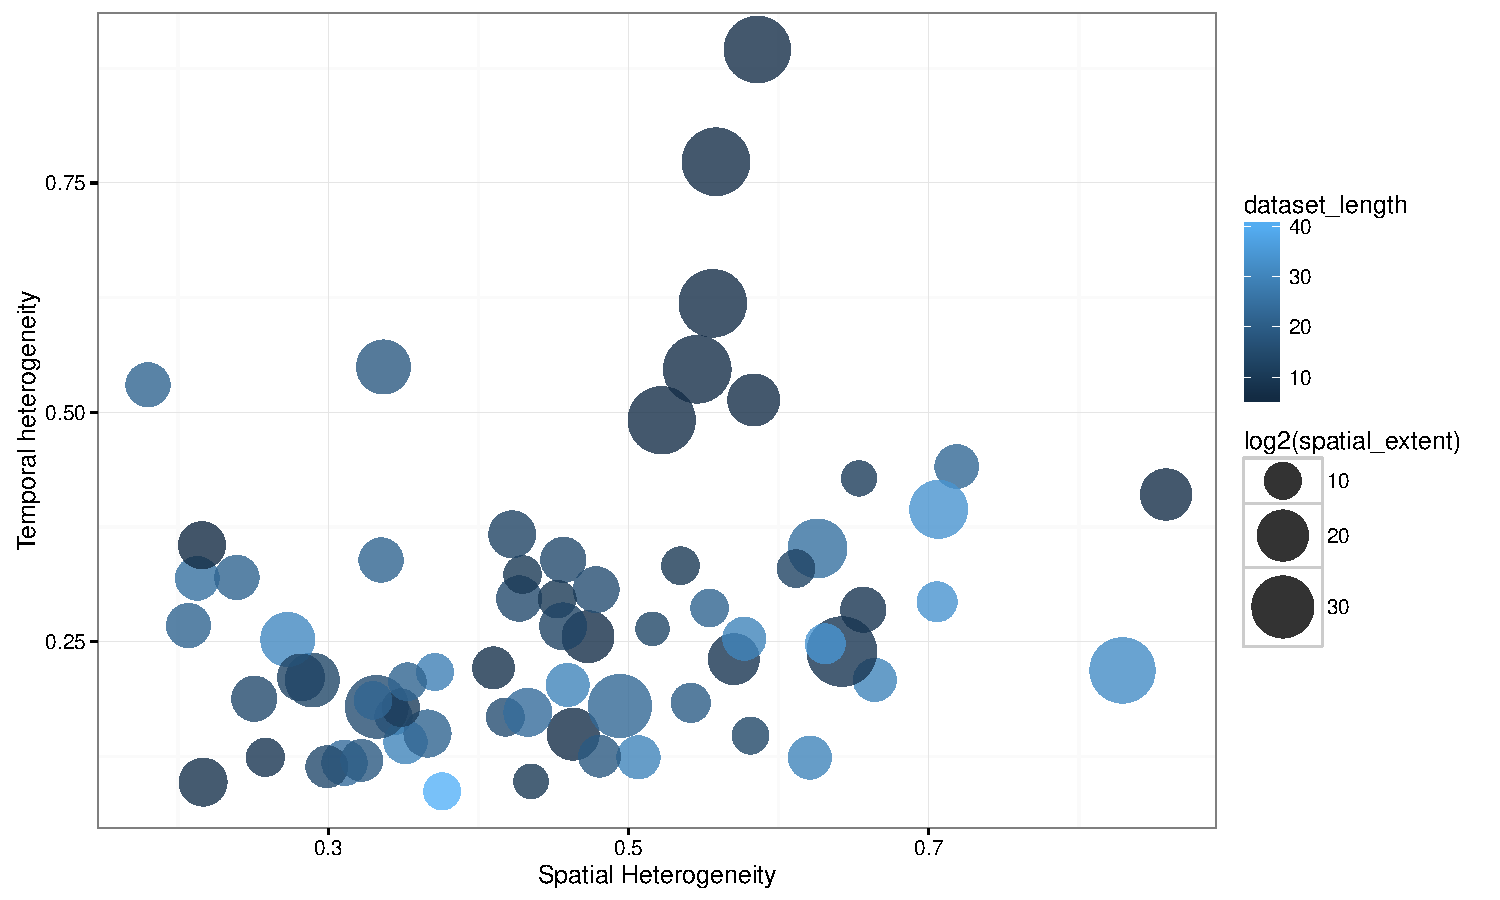
\includegraphics[width=400px]{overallagg}



\newpage
Difference between aquatic and terrestrial studies

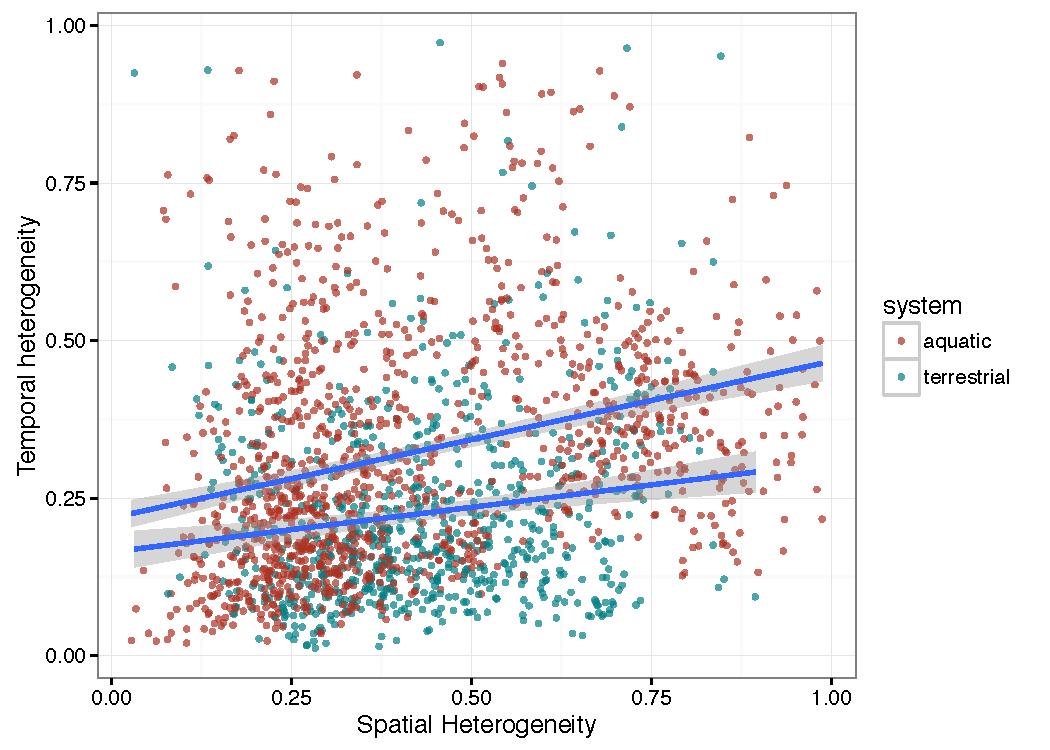
\includegraphics[width=400px]{aqterr}
\newpage

Table 1. Summary of mixed effect model of spatial heterogeneity on temporal heterogeneity, with study design features as covariates

\FloatBarrier
\begin{table}[ht]
\centering
\begin{tabular}{rrrr}
  \hline
 & Estimate & Std. Error & t value \\ 
  \hline
(Intercept) & 0.29 & 0.07 & 4.00 \\ 
  dispersion & 0.23 & 0.08 & 3.00 \\ 
  plot\_size & -0.00 & 0.00 & -0.66 \\ 
  num\_plots & 0.00 & 0.00 & 0.73 \\ 
  spatial\_extent & -0.00 & 0.00 & -0.37 \\ 
  dataset\_length & -0.00 & 0.00 & -1.79 \\ 
  time\_step & -0.07 & 0.04 & -1.67 \\ 
   \hline
\end{tabular}
\end{table}
\FloatBarrier



Figure 4. Summary of mixed-effect model for study design features 

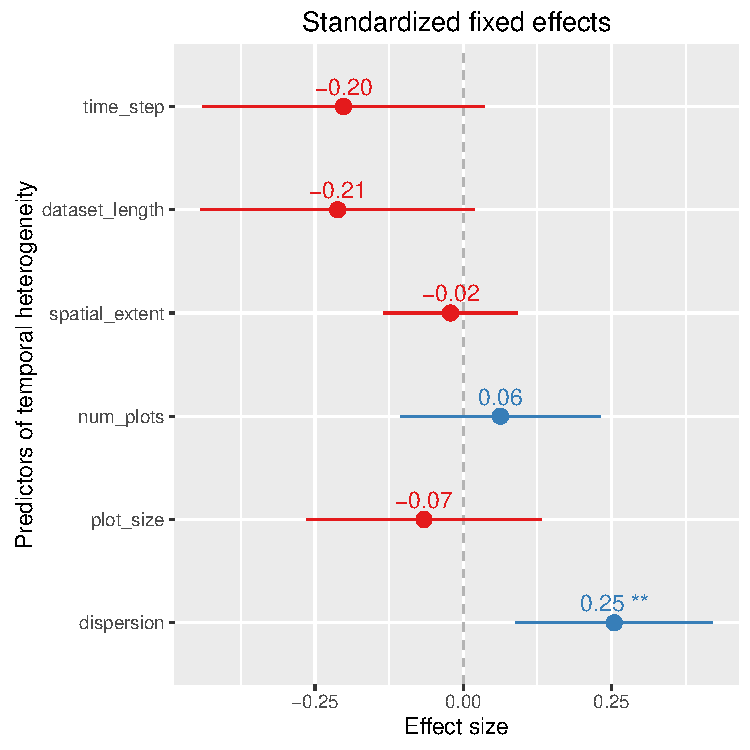
\includegraphics[width=300px]{designmodel}
\pagebreak


Table 2. System and organism-level features as covariates of effect of spatial heterogeneity on temporal heterogeneity

\FloatBarrier
\begin{table}[ht]
\centering
\begin{tabular}{rrrr}
  \hline
 & Estimate & Std. Error & t value \\ 
  \hline
(Intercept) & 0.05 & 0.15 & 0.35 \\ 
  dispersion & 0.33 & 0.08 & 3.99 \\ 
  taxainvertebrates & 0.16 & 0.17 & 0.95 \\ 
  taxaphytoplankton & 0.18 & 0.17 & 1.03 \\ 
  taxaplants & 0.12 & 0.17 & 0.72 \\ 
  taxazooplankton & 0.12 & 0.15 & 0.78 \\ 
  lifespanlonger & -0.07 & 0.04 & -1.62 \\ 
  S & 0.00 & 0.00 & 0.64 \\ 
  ANPP & -0.00 & 0.00 & -0.43 \\ 
  successionyes & 0.05 & 0.03 & 1.84 \\ 
  systemterrestrial & -0.06 & 0.10 & -0.55 \\ 
   \hline
\end{tabular}
\end{table}
\FloatBarrier

Figure 5. Summary of mixed-effect model for taxonomic and ecosystem type system features 

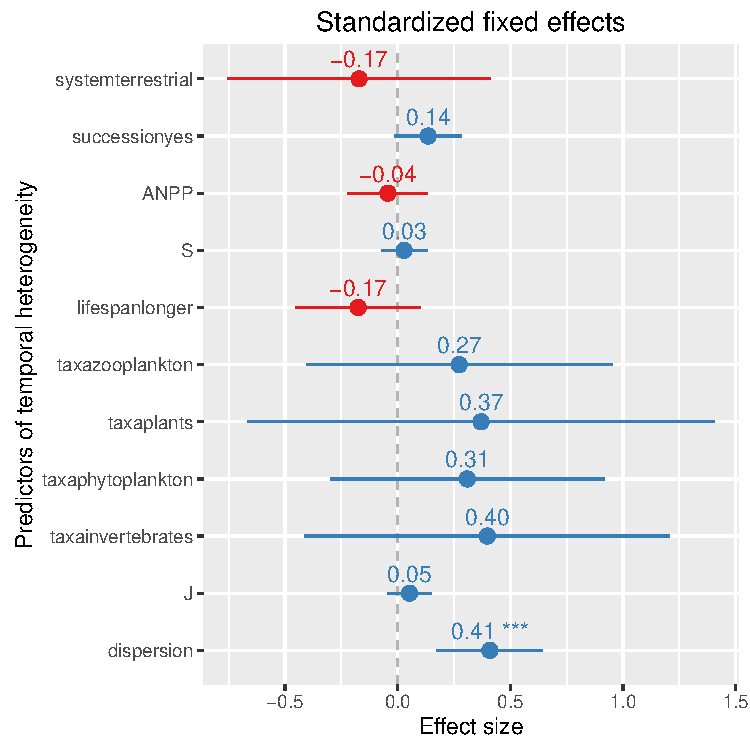
\includegraphics[width=280px]{systemmodel}



\end{document}